\section*{Exploration numérique}
\phantomsection
\addcontentsline{toc}{section}{Exploration numérique}

\subsection*{Question 1 — départ en état 2}
\phantomsection
\addcontentsline{toc}{subsection}{Question 1 — départ en état 2}
Nous allons calculer \(\Pi^{(n)} = \Pi^{(0)} M^{n}\) avec \(\Pi^{(0)} = e_2\) (vecteur unité en position 2 pour commencer à l'état 2) et \(M\) la matrice 27\(\times\)27 fournie.
Nous allons utiliser le programme réalisé en projet de C \texttt{markov\_analyzer} \parencite{markovGraphAnalyzer2025} qui va  reconstruire d'abord la matrice de transition \(M\) à partir du fichier fourni sur Moodle, puis calculer les distributions \(\Pi^{(n)}\) pour \(n=1,2,10,50\).
\begin{itemize}[label=\textbullet]
  \item Arguments utilisés : \\
  \texttt{./markov\_analyzer -{}-in data/moodle/matrix.txt -{}-dist-start 2 -{}-dist-steps 1} \\
  \texttt{./markov\_analyzer -{}-in data/moodle/matrix.txt -{}-dist-start 2 -{}-dist-steps 2} \\
  \texttt{./markov\_analyzer -{}-in data/moodle/matrix.txt -{}-dist-start 2 -{}-dist-steps 10} \\
  \texttt{./markov\_analyzer -{}-in data/moodle/matrix.txt -{}-dist-start 2 -{}-dist-steps 50}
  \item Les sorties détaillées sont disponibles dans \texttt{data/q1/n\{1,2,10,50\}\_out.txt}; un calcul supplémentaire à \(n=51\) (\texttt{n51\_out.txt}) sert pour le test de convergence \(\Pi^{(n+1)} - \Pi^{(n)}\).
\end{itemize}

\paragraph{(a) Distributions des probabilités :} Les composantes non nulles sont rassemblées dans le tableau~\ref{tab:q1_distributions} ;
les produits \(\Pi^{(0)} P^{n}\) sont effectués avec les fonctions \texttt{dist\_step}\textsuperscript{\ref{lst:dist_step}} et \texttt{dist\_power}\textsuperscript{\ref{lst:dist_power}}.
\begin{table}[H]
  \centering
  \begin{tabular}{@{}lccccc@{}}
    \toprule
    \(n\) & \(\Pi^{(n)}(2)\) & \(\Pi^{(n)}(5)\) & \(\Pi^{(n)}(12)\) & \(\Pi^{(n)}(21)\) & \(\Pi^{(n)}(25)\) \\
    \midrule
    1  & 0.30   & 0.20   & 0.40   & 0.00   & 0.10   \\
    2  & 0.23   & 0.22   & 0.28   & 0.17   & 0.10   \\
    10 & 0.2397 & 0.1953 & 0.2338 & 0.1796 & 0.1516 \\
    50 & 0.2397 & 0.1953 & 0.2338 & 0.1796 & 0.1516 \\
    \bottomrule
  \end{tabular}
  \caption{Distributions \(\Pi^{(n)}\) (départ en \(e_2\)), issues de \texttt{data/q1/n\{1,2,10,50\}\_out.txt}.}
  \label{tab:q1_distributions}
\end{table}

\paragraph{(b) Graphe \(n \mapsto \Pi_A(n)\).} La figure~\ref{fig:q1_pi} trace les cinq composantes non nulles pour \(n \in \{1,2,10,50\}\) (les autres restent à 0), avec un axe des abscisses en échelle logarithmique (base 10) pour mettre en évidence les premiers pas et les itérations lointaines.
On observe un lissage rapide autour de \(n\approx 10\).

\begin{figure}[H]
  \centering
  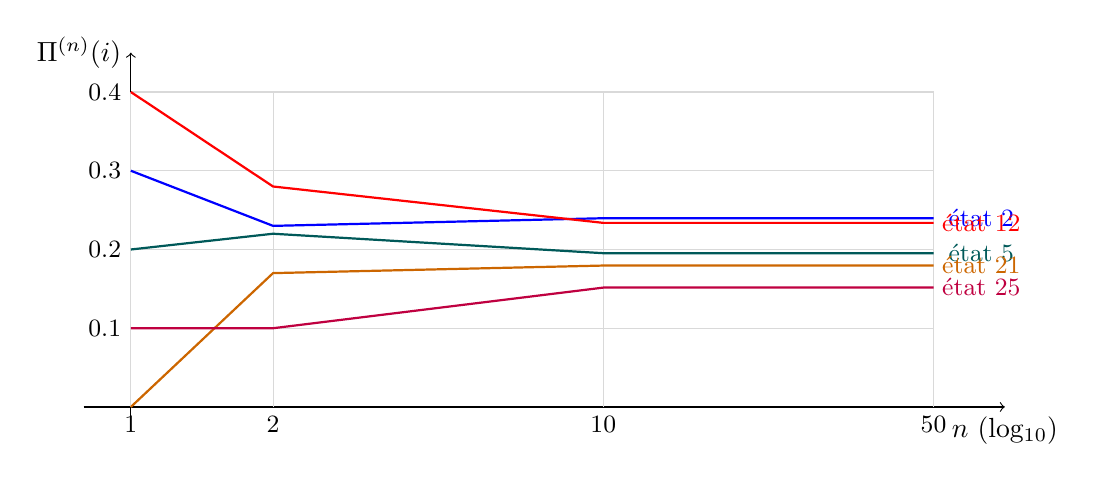
\begin{tikzpicture}[xscale=6,yscale=10]
    % Axes
    \draw[->] (-0.1,0) -- (1.85,0) node[below] {$n$ (log\textsubscript{10})};
    \draw[->] (0,-0.02) -- (0,0.45) node[left] {$\Pi^{(n)}(i)$};
    % Grille et repères (log10)
    \foreach \x/\lbl in {0/{\small 1},0.3010/{\small 2},1/{\small 10},1.6990/{\small 50}}{
      \draw[gray!30] (\x,0) -- (\x,0.4);
      \node[below] at (\x,0) {\lbl};
    }
    \foreach \y in {0.1,0.2,0.3,0.4}{\draw[gray!30] (0,\y) -- (1.7,\y); \node[left] at (0,\y) {\small \y};}
    % Etat 2
    \draw[blue,thick] plot coordinates {(0,0.3) (0.3010,0.23) (1,0.2397) (1.6990,0.2397)};
    \node[blue] at (1.8,0.24) {\small état 2};
    % Etat 12
    \draw[red,thick] plot coordinates {(0,0.4) (0.3010,0.28) (1,0.2338) (1.6990,0.2338)};
    \node[red] at (1.8,0.234) {\small état 12};
    % Etat 5
    \draw[teal!70!black,thick] plot coordinates {(0,0.2) (0.3010,0.22) (1,0.1953) (1.6990,0.1953)};
    \node[teal!70!black] at (1.8,0.196) {\small état 5};
    % Etat 21
    \draw[orange!80!black,thick] plot coordinates {(0,0.0) (0.3010,0.17) (1,0.1796) (1.6990,0.1796)};
    \node[orange!80!black] at (1.8,0.18) {\small état 21};
    % Etat 25
    \draw[purple,thick] plot coordinates {(0,0.1) (0.3010,0.1) (1,0.1516) (1.6990,0.1516)};
    \node[purple] at (1.8,0.152) {\small état 25};
  \end{tikzpicture}
  \caption{Évolution des composantes non nulles \(\Pi^{(n)}(i)\) (départ en \(e_2\)).}
  \label{fig:q1_pi}
\end{figure}

\paragraph{(c) Existence et valeur de la distribution limite.} Le calcul supplémentaire à \(n=51\) (\texttt{data/q1/n51\_out.txt}) donne \(\Pi^{(51)} = \Pi^{(50)}\) à \(10^{-4}\) près, donc \(\Pi^{(51)} - \Pi^{(50)} \approx 0\) pour chaque composante.
La distribution limite est donc atteinte à \(n=50\) avec les valeurs suivantes :
\begin{align*}
  \Pi^{(\infty)}(2)&=0{,}2397, & \Pi^{(\infty)}(5)&=0{,}1953, \\
  \Pi^{(\infty)}(12)&=0{,}2338, & \Pi^{(\infty)}(21)&=0{,}1796, \\
  \Pi^{(\infty)}(25)&=0{,}1516,
\end{align*}
et les autres composantes nulles.

\subsection*{Question 2 — répartition uniforme sur 2, 5, 12, 21, 25}
\phantomsection
\addcontentsline{toc}{subsection}{Question 2 — répartition uniforme sur 2, 5, 12, 21, 25}
Pour répondre à cette question, nous avons vérifié si la distribution limite dépendait de l'état de départ parmi l'ensemble \(\{2, 5, 12, 21, 25\}\). Nous avons exécuté notre programme pour chacun de ces états avec \(n=50\) (car nous avions déduit une limite à \(n=50\) pour l'état 2):
\begin{itemize}[label=\textbullet]
    \item \texttt{./markov\_analyzer -{}-in data/moodle/matrix.txt -{}-dist-start 5 -{}-dist-steps 50}
    \item \texttt{./markov\_analyzer -{}-in data/moodle/matrix.txt -{}-dist-start 12 -{}-dist-steps 50}
    \item \texttt{./markov\_analyzer -{}-in data/moodle/matrix.txt -{}-dist-start 21 -{}-dist-steps 50}
    \item \texttt{./markov\_analyzer -{}-in data/moodle/matrix.txt -{}-dist-start 25 -{}-dist-steps 50}
\end{itemize}
Les résultats numériques (fichiers \texttt{data/q2\_q3/from\_*.txt}) montrent que pour tous ces états, la distribution à \(n=50\) est \textbf{identique} à celle obtenue pour l'état 2 (Question 1).
Voici les valeurs obtenues (on assimile \(\Pi^{(50)}\) à \(\Pi^{(\infty)}\) car la convergence a été établie à \(10^{-4}\) près dès \(n=50\) à la question 1) :

\begin{table}[H]
    \centering
    \begin{tabular}{@{}lccccc@{}}
        \toprule
        État \(i\) & 2 & 5 & 12 & 21 & 25 \\
        \midrule
        \(\Pi^{(\infty)}(i)\) & 0.2397 & 0.1953 & 0.2338 & 0.1796 & 0.1516 \\
        \bottomrule
    \end{tabular}
    \caption{Distribution limite commune pour les états de départ \{2, 5, 12, 21, 25\}.}
    \label{tab:q2_limit}
\end{table}

Puisque la distribution initiale est uniforme (\(\Pi^{(0)} = \frac{1}{5}e_2 + \frac{1}{5}e_5 + \frac{1}{5}e_{12} + \frac{1}{5}e_{21} + \frac{1}{5}e_{25}\)), par linéarité de la multiplication matricielle :
\[
\Pi^{(\infty)} = \frac{1}{5}\Pi^{(\infty)}_2 + \frac{1}{5}\Pi^{(\infty)}_5 + \frac{1}{5}\Pi^{(\infty)}_{12} + \frac{1}{5}\Pi^{(\infty)}_{21} + \frac{1}{5}\Pi^{(\infty)}_{25} = \frac{1}{5}(5 \times \Pi_{lim}) = \Pi_{lim}
\]
\textbf{Conclusion :} Il existe une distribution limite, et c'est exactement la même que celle trouvée à la Question 1.

\subsection*{Question 3 — répartition aléatoire sur 2, 5, 12, 21, 25}
\phantomsection
\addcontentsline{toc}{subsection}{Question 3 — répartition aléatoire sur 2, 5, 12, 21, 25}
Soit une distribution initiale aléatoire répartie sur ces mêmes états :
\[
\Pi^{(0)} = a e_2 + b e_5 + c e_{12} + d e_{21} + e e_{25} \quad \text{avec} \quad a+b+c+d+e=1
\]
Nous avons établi expérimentalement que \(\lim_{n \to \infty} e_i M^n = \Pi_{lim}\) pour tout \(i \in \{2, 5, 12, 21, 25\}\).
Par linéarité :
\[
\lim_{n \to \infty} \Pi^{(0)} M^n = a \Pi_{lim} + b \Pi_{lim} + c \Pi_{lim} + d \Pi_{lim} + e \Pi_{lim} = (a+b+c+d+e) \Pi_{lim} = \Pi_{lim}
\]
\textbf{Conclusion :} La distribution limite existe et est \textbf{indépendante} des paramètres initiaux \(a, b, c, d, e\). Elle reste identique à celle de la Question 1.

\subsection*{Question 4 — états 8, 9, 16}
\phantomsection
\addcontentsline{toc}{subsection}{Question 4 — états 8, 9, 16}
\placeholder{Comparer départ en 8 vs. mélange uniforme vs. mélange aléatoire.}

\subsection*{Question 5 — états 10, 14, 19, 22, 24}
\phantomsection
\addcontentsline{toc}{subsection}{Question 5 — états 10, 14, 19, 22, 24}
\placeholder{Identifier les comportements limites selon les trois répartitions demandées.}

\subsection*{Question 6 — états 6, 17, 20}
\phantomsection
\addcontentsline{toc}{subsection}{Question 6 — états 6, 17, 20}
\placeholder{Documenter les trajectoires de \(\Pi^{(n)}\) et la présence/absence de limite.}

\subsection*{Question 7 — états 3, 7, 23}
\phantomsection
\addcontentsline{toc}{subsection}{Question 7 — états 3, 7, 23}
\placeholder{Même analyse : convergence éventuelle et dépendance à l'initialisation.}
